\setlength{\parskip}{\baselineskip} 
%\section{\bnmf}

\frame{
	\frametitle{\bnmf application}
\begin{columns}
\column{0.6\textwidth}
\vspace{1em}
\begin{itemize}
    \item {\color{matbluedark}\textbf{Study Population}}
    \begin{itemize}
        \item Mothers \& Newborns cohort
        \item N = 343 pregnant women
    \end{itemize}
    \item {\color{matbluedark}\textbf{Mixture of interest}} 
    \begin{itemize}
        \item Endocrine disrupting chemicals
        \item 9 phthalate metabolites
        \item 8 phenols
    \end{itemize}
    \item {\color{matbluedark}\textbf{Research questions}} 
    \begin{itemize}
        \item Are there patterns of EDC exposure?
        \item Are identified patterns associated with child intelligence?
    \end{itemize}
\end{itemize}
\column{0.5\textwidth}
\centering
\includegraphics[scale=0.4]{figures/ccceh_logo.jpg}
%\vspace{-4ex}
\end{columns}
}

\frame{\frametitle{\bnmf application: EDC correlation}
\vspace{-3.5em}
\begin{center}
	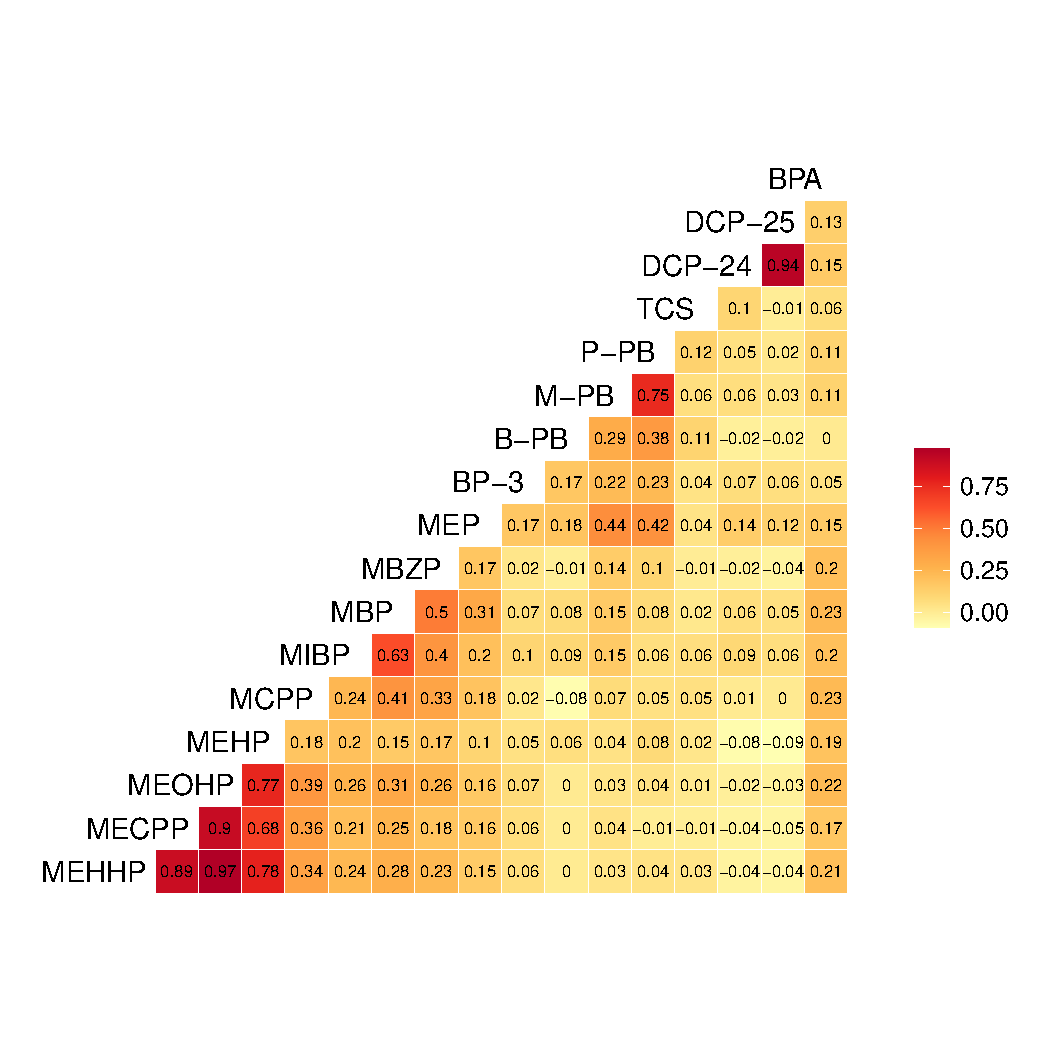
\includegraphics[scale=0.54]{figures/bn2mf/ppp_corr_prez.pdf}
\end{center}
}

\frame{\frametitle{Mothers \& Newborns results: 2 underlying patterns of EDC exposure}
\vspace{5ex}
\hspace{-1em}	
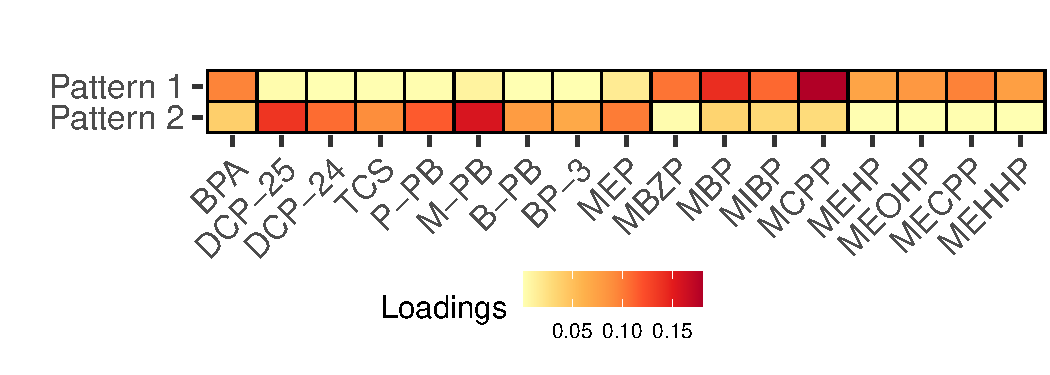
\includegraphics[scale=0.65]{figures/bn2mf/prez_eh_loadings.pdf}
}

\frame{
	\frametitle{Patterns represent known exposure sources}
\vspace{1.75em}
\begin{changemargin}{-1.5em}{-1.5em}
\begin{columns}
\column{0.5\textwidth}
\vspace{-1.5em}
\LARGE
\begin{center}
Pattern 1:
\end{center}
\column{0.5\textwidth}
\vspace{-1.5em}
\LARGE
\begin{center}
Pattern 2:
\end{center}
\end{columns}
\end{changemargin}
\vspace{1ex}
\begin{changemargin}{-1.5em}{-1.5em}
\begin{columns}
\column{0.5\textwidth}
\LARGE
\begin{tcolorbox}[boxsep=-1ex,boxrule=2pt,colframe=matbluedark, colback=white,height=4.75cm]
\begin{center}
\vspace{1ex}
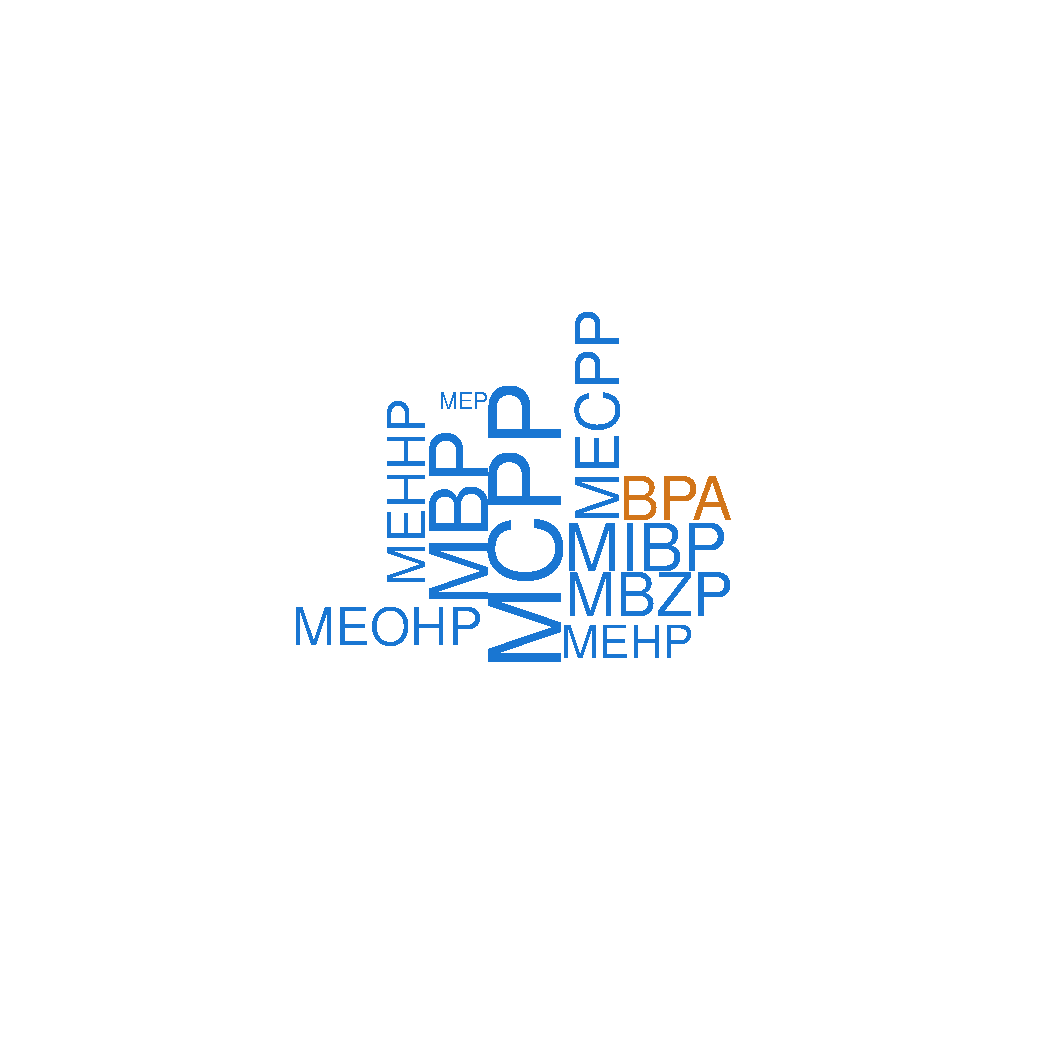
\includegraphics[height=4.25cm]{figures/bn2mf/cloud1.pdf}
\end{center}
\end{tcolorbox}
\column{0.5\textwidth}
\LARGE
\begin{tcolorbox}[boxsep=-1ex,boxrule=2pt,colframe=cloudorange, colback=white,height=4.75cm]
\begin{center}
\vspace{1ex}
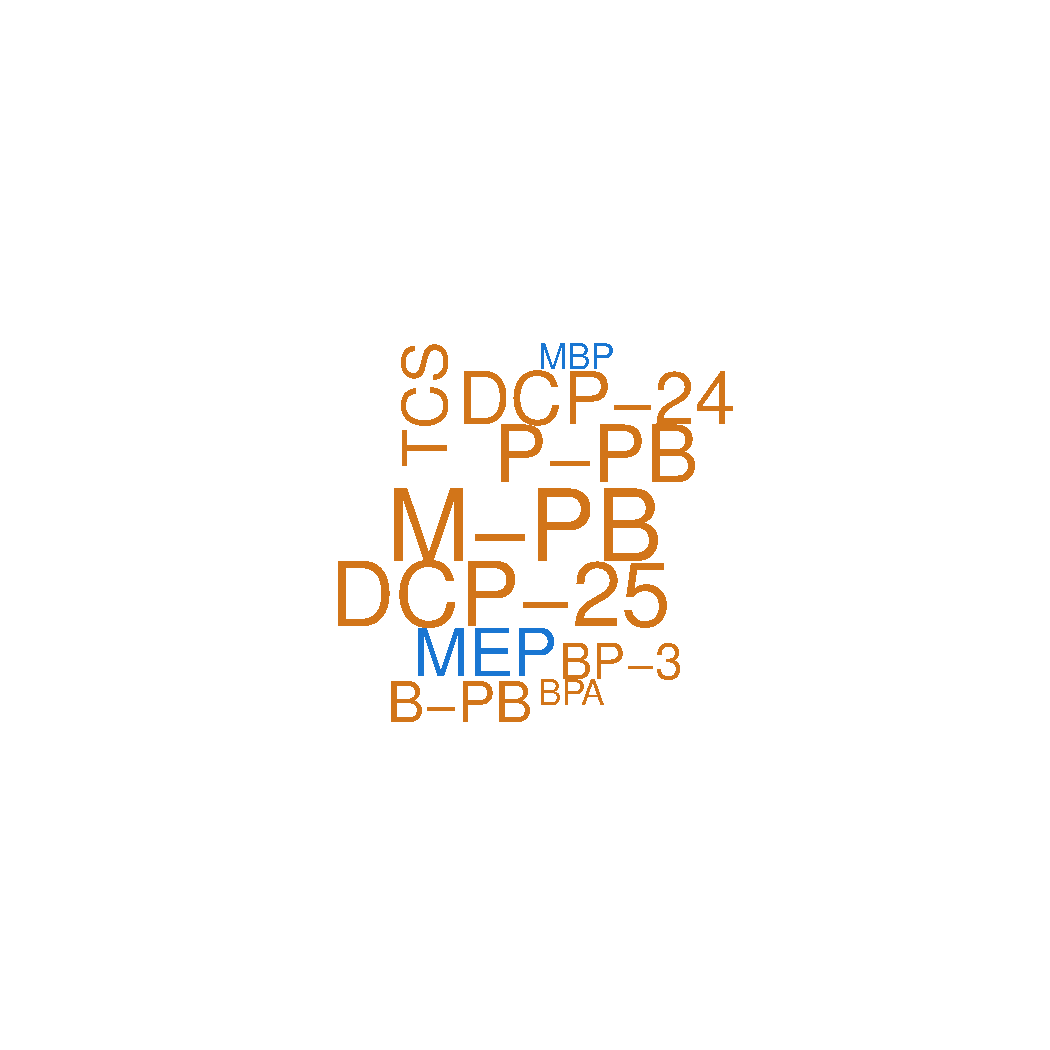
\includegraphics[height=4.25cm]{figures/bn2mf/cloud2.pdf}
\end{center}
\end{tcolorbox}
\end{columns}
\end{changemargin}
\vspace{0.5ex}
\begin{changemargin}{-1.5em}{-1.5em}
\begin{columns}[b]
\column{0.5\textwidth}
\LARGE
\begin{center}
\large
\includesvg[scale=0.03]{figures/bn2mf/canned-food.svg}  {Food packaging}  \includesvg[scale=0.03]{figures/bn2mf/canned-food.svg}
\end{center}
\column{0.5\textwidth}
\large
\begin{center}
\includesvg[scale=0.03]{figures/bn2mf/shampoo-svgrepo-com.svg}  {Personal care products}  \includesvg[scale=0.03]{figures/bn2mf/shampoo-svgrepo-com.svg}
\end{center}
\end{columns}
\end{changemargin}
\vspace{-1em}
\begin{center}
\tiny
\textbf{{\color{matbluedark}\bullet \ Phthalates} \
{\color{cloudorange}\bullet \ Phenols}}
\end{center}
}

\frame{
\frametitle{Bayesian non-parametric non-negative matrix factorization (BN$^{2}$MF)}
\begin{columns}
\column{.6\textwidth}
\ \\
\vspace{2em}
\centering\color{matbluedark}{\LARGE\texttt{\textbf{BIG PICTURE}}}
\vspace{.5\baselineskip}
\begin{itemize}
         \item Enhanced interpretability
         \begin{itemize}
	\item Parts-based (additive) {\color{matbluedark}non-negative} representation
    \item No orthogonality constraint
	\end{itemize}
         \item Non-parametric prior chooses the number of patterns
         \item Quantifies uncertainty
         \begin{itemize}
	\item[\rightarrow] To propagate into health model
	\end{itemize}
        \end{itemize}
\column{.4\textwidth}
\ \\
\vspace{2em}
\centering\includesvg[scale=0.35]{figures/robot-svgrepo-com.svg}
\end{columns}
}